\part{História do Jogo}

\section{Como e aonde começa o jogo}

O jogo não possue uma grande história tomando como base que a finalidade dele é apenas passar a fase imposta. O jogo inicia com o carro centralizado na pista atrás da linha de partida, o jogador tem que esperar o tempo regressivo de 3 segundos acabar para começar a correr.

\section{Cenários do jogo e suas inter-relações}

A ideia geral do jogo seria ir passando das fases tendo uma sequência de paisagens, por conta das restrições de tempo, base e conhecimento, a ideia central é, com o auxílio do Blender, Unity e as linguagens, fazer apenas uma fase. A fase \'e um cen\'ario com montanhas, \'arvores, grama verde e uma cachoeira em um lugar isolado.

O modelo de cen\'ario ser\'a parececido com o modelo teste deste v\'ideo,  \href{https://www.youtube.com/watch?v=9V2GcBU732g}{YouTube}.

\section{Troca de cen\'arios}

Como o jogo em quest\~ao ter\'a apenas uma fase, não haverá troca de cenário.

\section{Final do Jogo}

Ao final da fase, terá uma bandeira de linha de chegada. Quando o jogador chegar a linha, o jogo encerra mostrando ao usu\'ario uma tabela com as informações de tempo de corrida, sua colocação no rank principal e uma opção de voltar a tela inicial e outra de reiniciar a corrida.

\begin{figure}[!h]
	\centering
		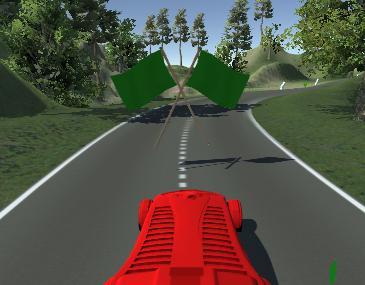
\includegraphics[scale=0.5]{figuras/final}
	\caption{Imagem da tela final}
\end{figure}

\section{Como chegar ao final}

O jogador terá que passar por toda a fase realizando as ações impostas que são: coletar os nitros não deixando o combustível acabar e se mantendo dentro do percurso. Ao chegar na linha de chegada, o jogo encerra.